\chapter{Paso a tablas}

\section{Proceso de traducción}

\subsection{Traducción de entidades fuertes}

Para un conjunto de entidades fuertes $E$ con atributos $a_i$, podemos representar cada una de estas entidades mediante una tabla donde cada \textbf{tupla} (fila) es una instancia de la entidad y contiene tantas columnas como atributos contine la misma.
Los atributos que sean clave primaria se subrayan en el esquema resultante.
Opcionalmente, se puede escribir \textit{CP} debajo del subrayado.

\begin{figure}[h]
\begin{center}
	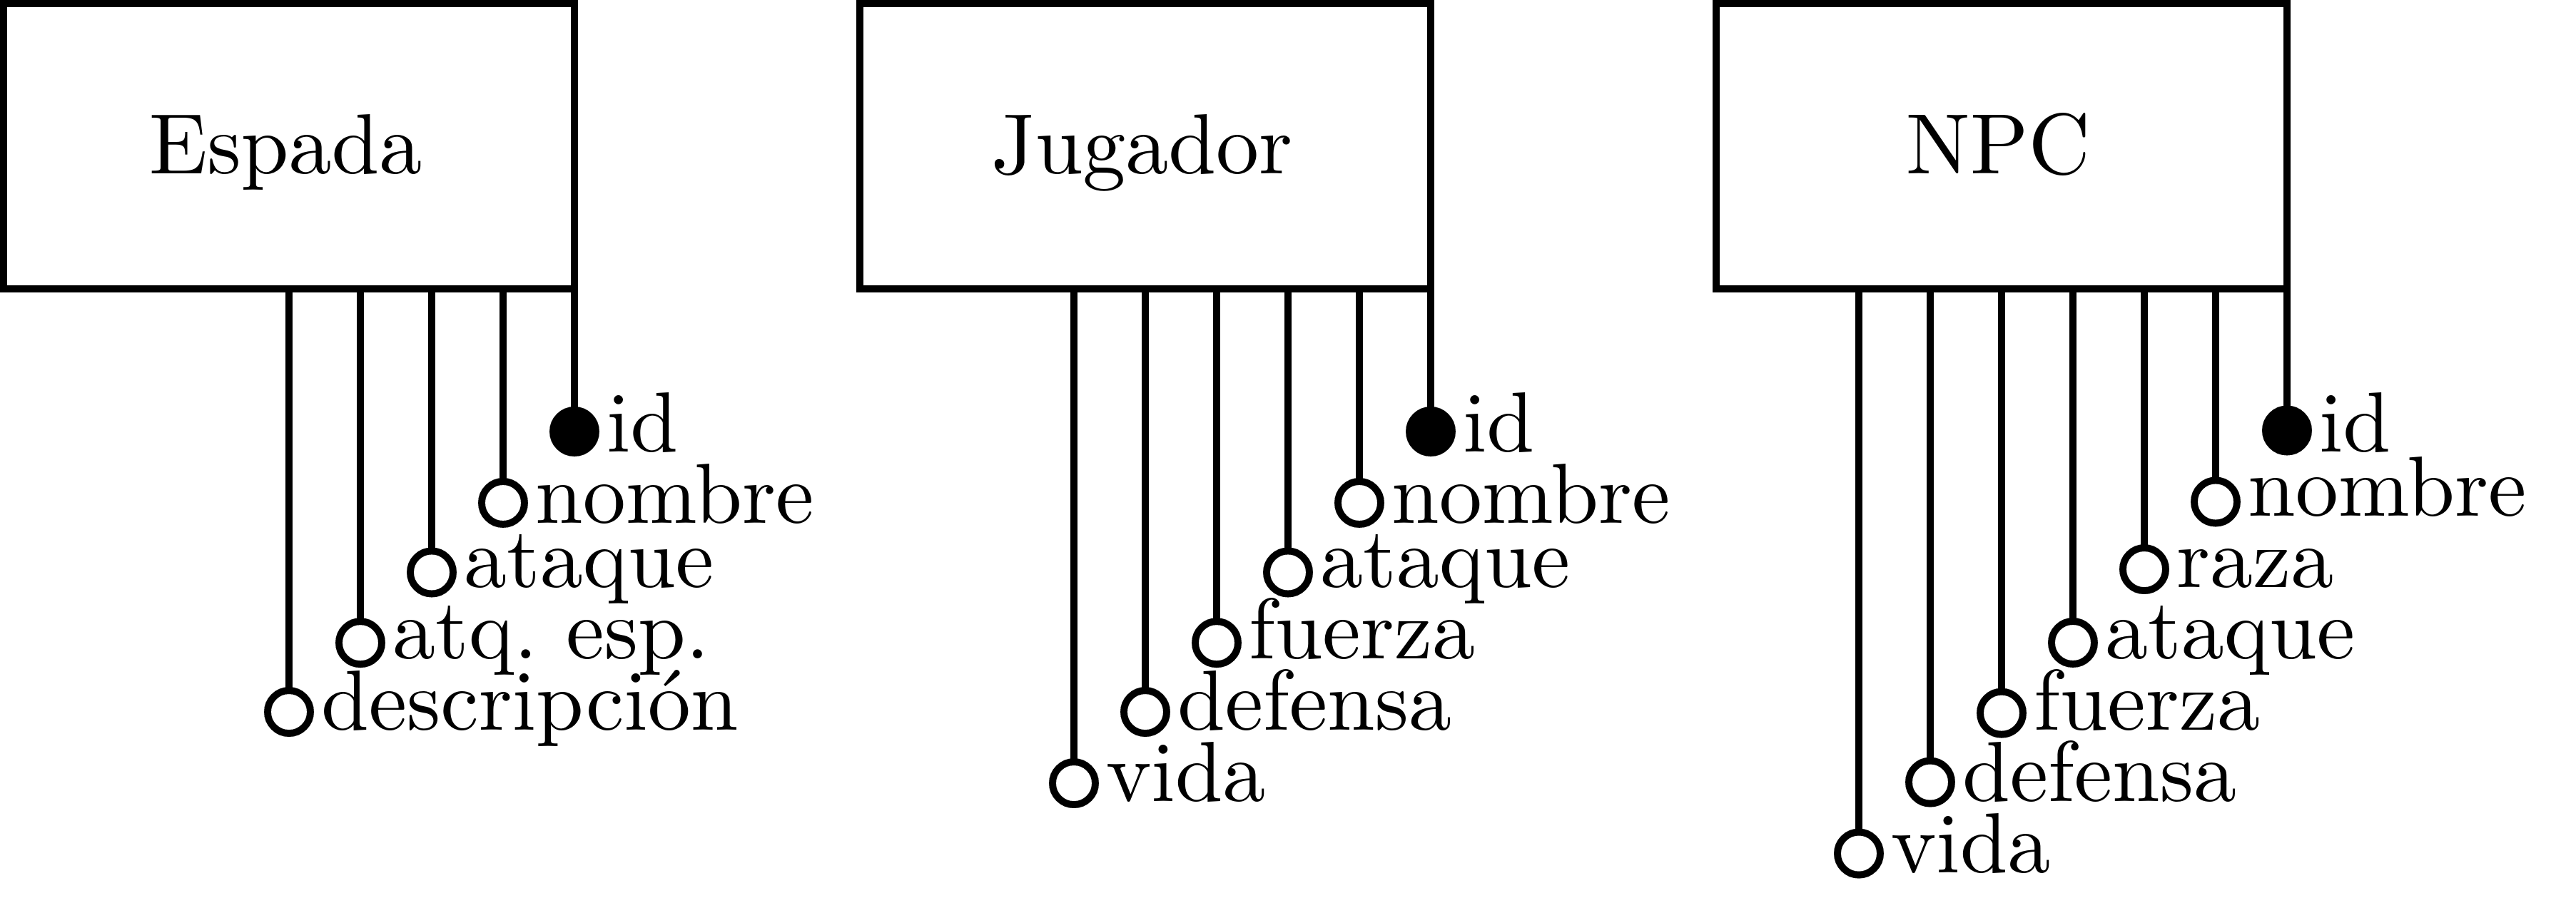
\includegraphics[scale=0.06]{EntidadesFuertes}
\end{center}
\caption{Ejemplo de tres entidades fuertes con atributos}
\end{figure}

Estas tres entidades se traducen en las siguientes tablas:

\begin{itemize}
	\item \textbf{Espada} (\underline{id}, nombre, ataque, atq\_esp, descripción)
	\item \textbf{Jugador} (\underline{id}, nombre, ataque, fuerza, defensa, vida)
	\item \textbf{NPC} (\underline{id}, nombre, raza, ataque, fuerza, defensa, vida)
\end{itemize}

\subsection{Traducción de entidades débiles}

Para un conjunto de entidades débiles $A$ con atributos $a_i$ y un conjunto de entidades fuertes $B$ del que dependen con atributos de clave primaria $b_i$, representamos $A$ por una tabla con las siguientes columnas:

\[\{a_i\forall a_k\in A\}\cup\{b_i\forall b_k\in B\}\]

La clave primaria de esta tabla está formada por la clave primaria de la entidad fuerte y los atributos discriminadores de la entidad débil.
Para relacionar correctamente ambas entidades, los atributos de entidad débil que referencien a la clave primaria de la entidad fuerte deben estar generados como \textbf{claves externas}, que podemos identificar con \textit{CE} de la misma forma que las claves primarias de las entidades fuertes.

\begin{figure}[h]
\begin{center}
	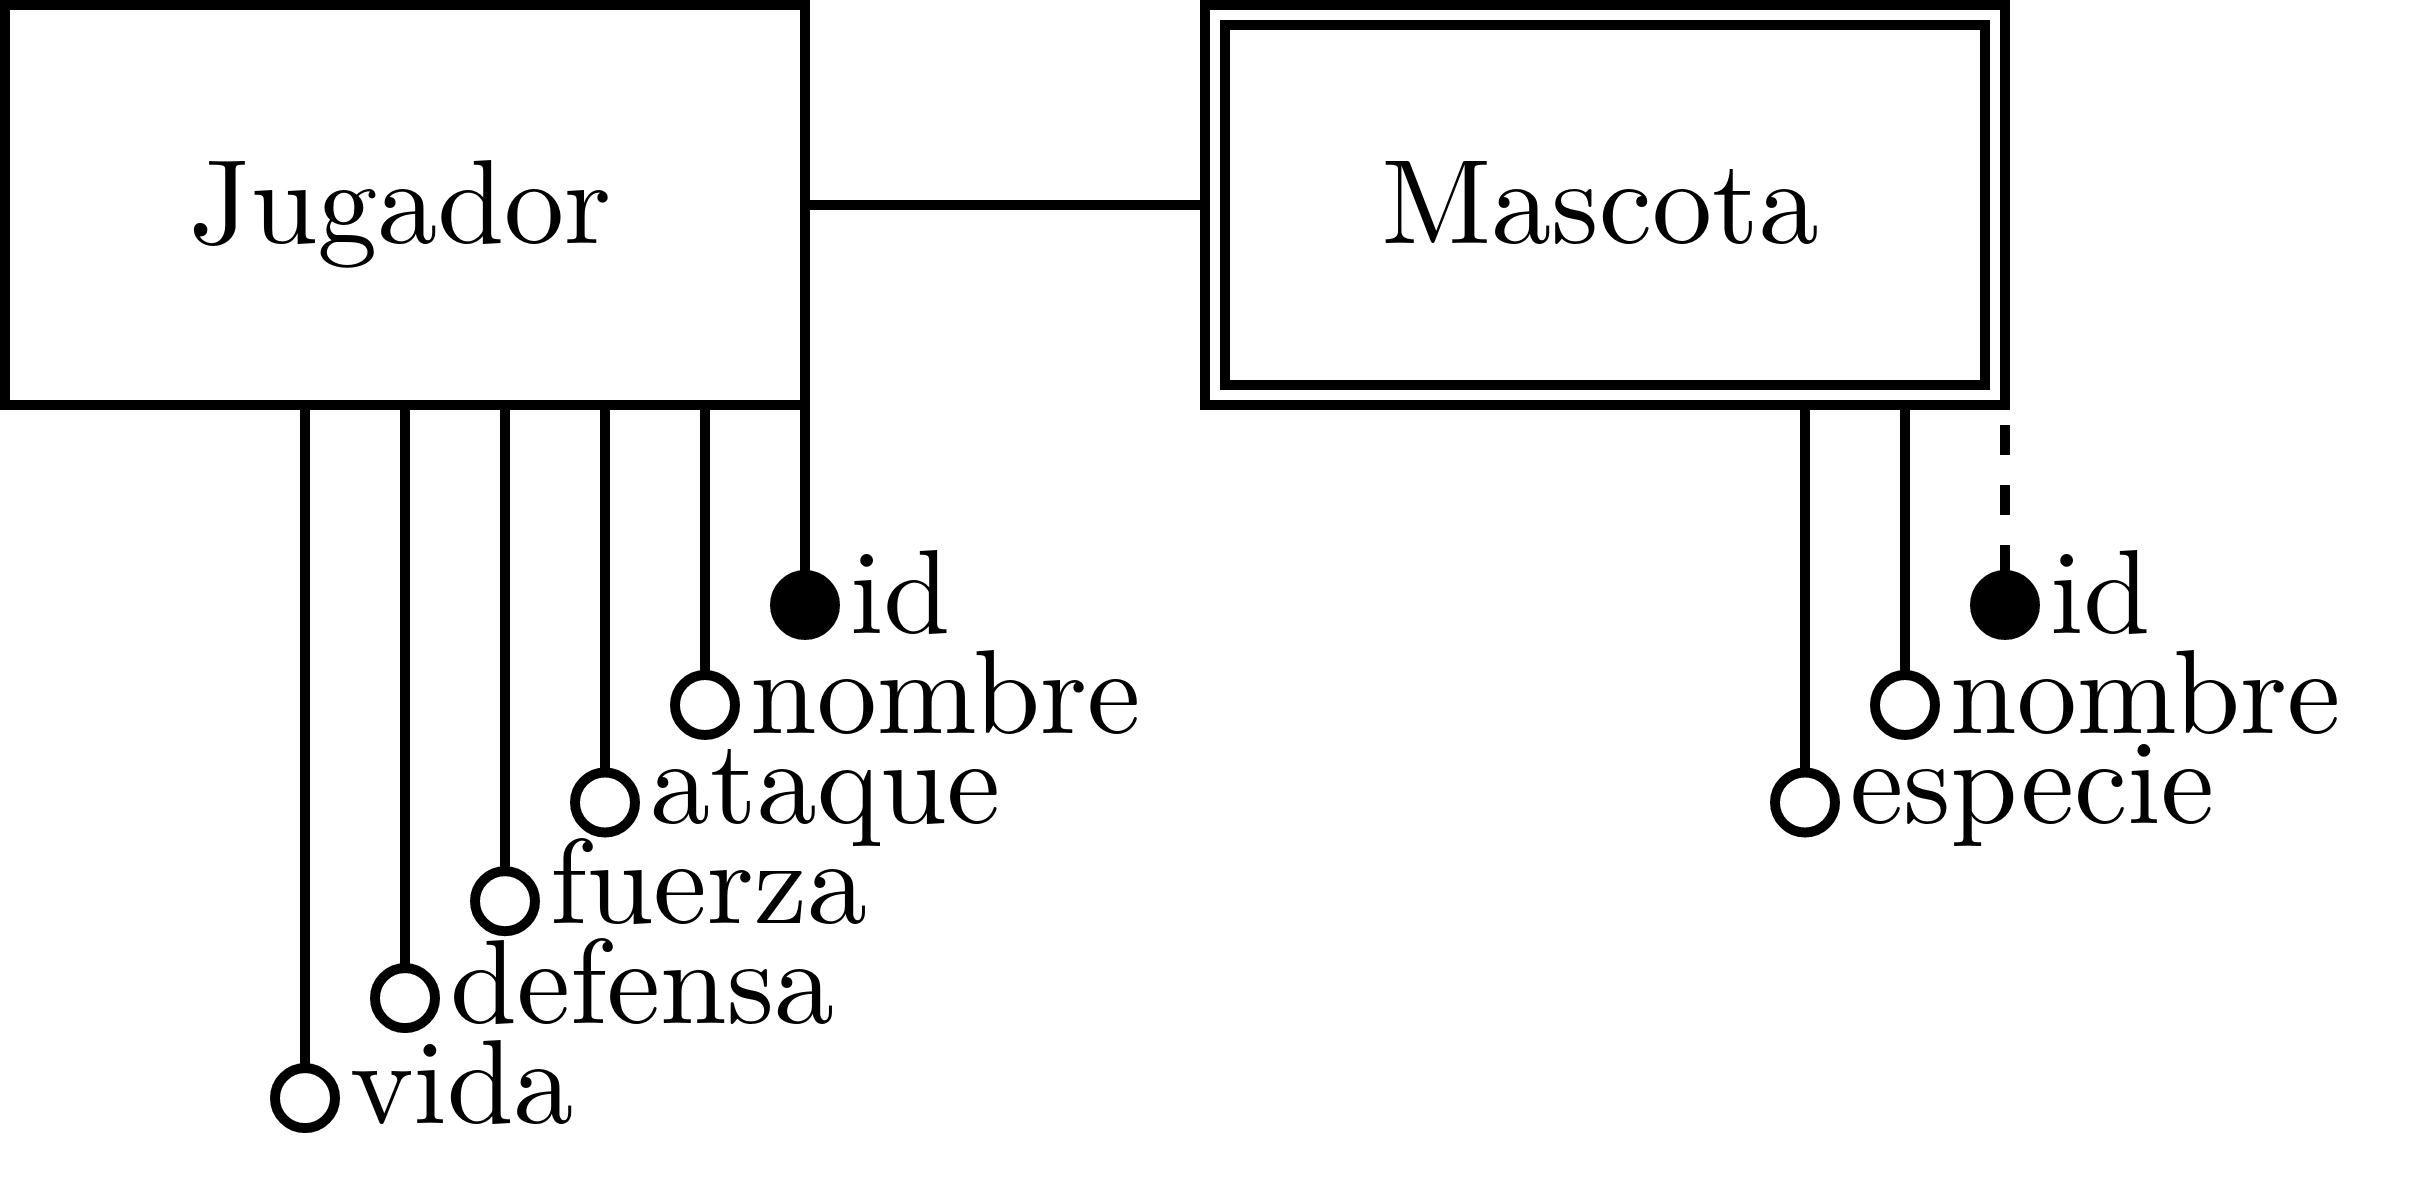
\includegraphics[scale=0.06]{EntidadDebil}
\end{center}
\caption{Entidad débil con su entidad fuerte}
\end{figure}

\pagebreak

Si la clave primaria de la entidad fuerte tiene el mismo nombre que el de la entidad débil (\code{id} en este caso), debemos cambiar el nombre de al menos una de ellas para distinguirlos.
El ejemplo anterior generaría estas dos tablas:

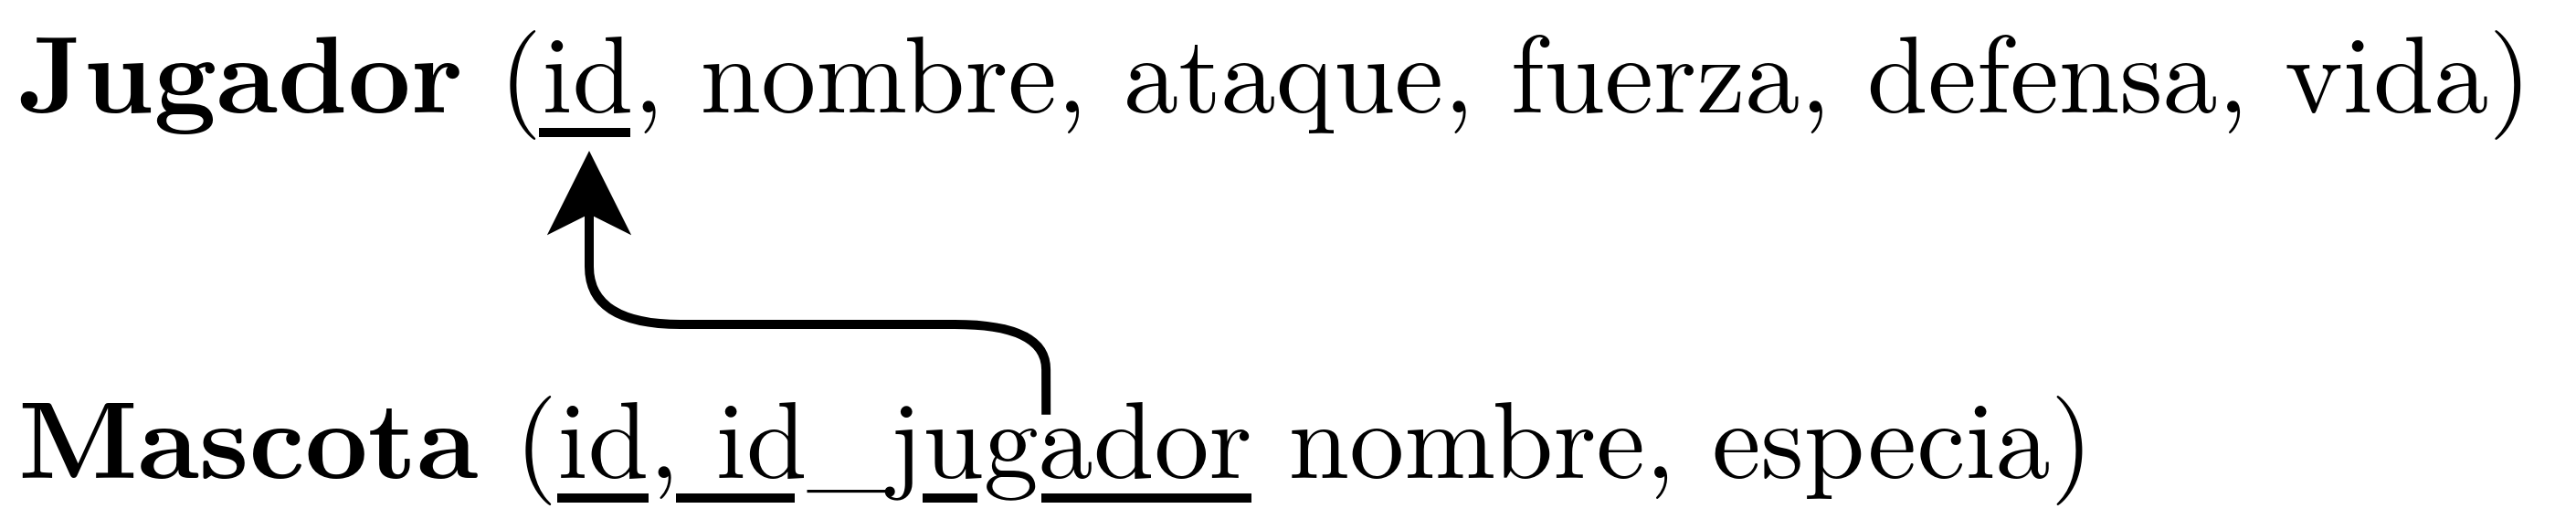
\includegraphics[scale=0.06]{TablaEntidadDebil}

\subsection{Traducción de una relación}

Para una relación $R$ que conecta un conjunto de entidades $E_i$,
